Consider a power grid with $C$ consumers and $G$ generators. We are interested
in connecting each consumer to a single generator, but each generator has a
limited capacity and the consumer draws a certain amount of power from the
generator. A valid powergrid is built in such a way that all consumers are
serviced by a generator and that no generator is being overdrawn by too many
consumers. Although consumers and generators may be connected through a complex
network, we analyze the simple case where any consumer is able to attach to any
generator.

\begin{wrapfigure}{r}{0.5\textwidth}
   \begin{center}
      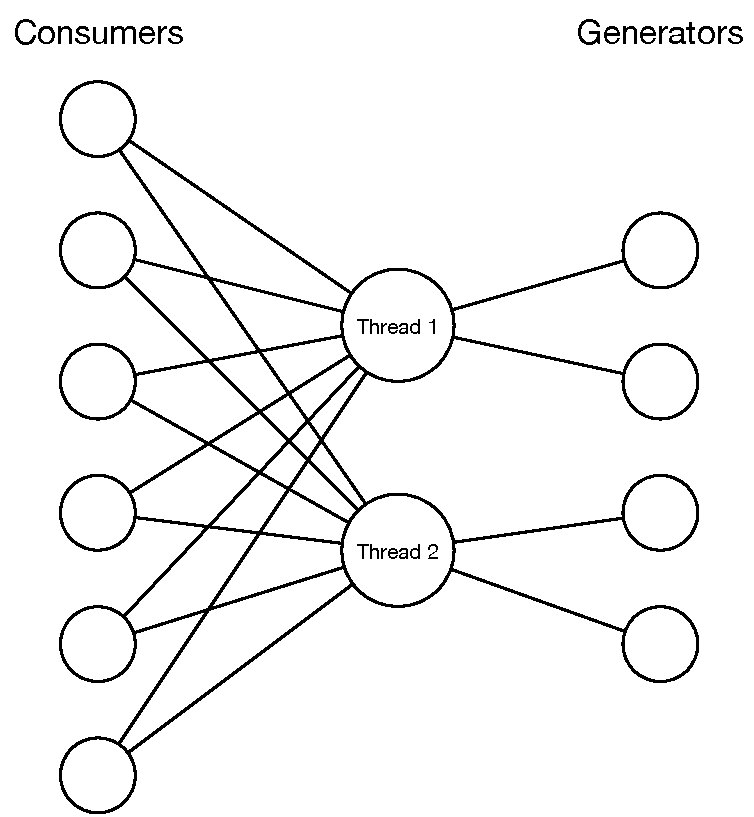
\includegraphics[width=1\linewidth]{figures/threads/powergrid.pdf}
   \end{center}
   \caption{Configuration of a powergrid with 6 consumers, 4
      generators and 2 threads, with each thread responsible for 2 generators.}
   \label{fig:threads:powergrid}
\end{wrapfigure}

A straightforward distributed implementation for the PowerGrid problem requires
that each consumer is able to connect to any generator. Once a generator
receives a connection request, it may or may not accept it. If the generator has
no power available for the new consumer, it will disconnect from it and the
consumer must select another generator. This randomized algorithm works but may
take a long time to converge, depending on the amount of power available in the
generators. Figure~\ref{code:threads:powergrid} shows the LM code for this
solution. Consumer and generators node types are declared in
lines~\ref{line:threads:pg_decl1}-\ref{line:threads:pg_decl2} using the
\code{node} declaration, allowing us to have different predicates for consumers
and generators. The \code{consumer} and \code{generator} types become a subtype
of \emph{node}, that is, $consumer <: node$ and $generator <: node$.  These
subtypes allow us to declare initial facts that only apply to either the
\code{consumer} or \code{generator} subtype.

\begin{figure}[h!]
\begin{Verbatim}[numbers=left,fontsize=\codesize,commandchars=*\#\&]
node generator.*label#line:threads:pg_decl1&*hfill// Type declaration
node consumer.*label#line:threads:pg_decl2&
type linear capacity(generator, int Total, int Used).*hfill// Predicate declaration
type linear connected-to(generator, consumer, int).
type linear connected-to-list(generator, list consumer).
type power(consumer, int).
type linear disconnected(consumer).
type linear connected(consumer, generator).
type generators(consumer, list generator).
type linear fails(generator, int).
type linear random-reconnect(generator).
type linear reconnect(consumer).
type linear connect(generator, consumer, int).
type linear disconnect(consumer, generator).

fails(G, Fails), Fails > maxfails*label#line:threads:pg_recon1&*hfill// Rule 1: disconnect one consumer
   -o random-reconnect(G).

capacity(G, Total, Used), random-reconnect(G),*hfill// Rule 2: disconnect one consumer
connected-to-list(G, L), L <> [], C = nth(L, randint(length(L))),
connected-to(G, C, Power)
   -o fails(G, 0), capacity(G, Total, Used - Power),
      connected-to-list(G, remove(L, C)), disconnect(C, G).

capacity(G, Total, Used), random-reconnect(G)*hfill// Rule 3: unable to disconnect one consumer
   -o capacity(G, Total, Used), fails(G, 0).*label#line:threads:pg_recon2&

connect(G, C, Power), capacity(G, Total, Used),*label#line:threads:pg_gen1&*hfill// Rule 4: connect consumer
fails(G, Fails), connected-to-list(G, L), Used + Power <= Total
   -o capacity(G, Total, Used + Power),
      fails(G, max(Fails - 1, 0)), connected-to(G, C, Power),
      connected-to-list(G, [C | L]).*label#line:threads:pg_gen2&

connect(G, C, Power), capacity(G, Total, Used),*label#line:threads:pg_fail1&*hfill// Rule 5: unable to connect consumer
Used + Power > Total, fails(G, Fails)
   -o capacity(G, Total, Used), disconnect(C, G),
      fails(G, Fails + 1).*label#line:threads:pg_fail2&

!generators(C, L), !power(C, Power),*label#line:threads:pg_connect1&*hfill// Rule 6: connect to a generator
reconnect(C), disconnected(C),
G = nth(L, randint(num-generators))
   -o connected(C, G), connect(G, C, Power).*label#line:threads:pg_connect2&

disconnect(C, G), connected(C, G)*hfill// Rule 7: finish disconnection
   -o disconnected(C), reconnect(C).

connected-to-list(G, []). fails(G, 0).*hfill// Initial facts
disconnected(C). reconnect(C). !generators(C, all-generators).
\end{Verbatim}
\caption{LM code for the regular PowerGrid program.}
\label{code:threads:powergrid}
\end{figure}

An example PowerGrid configuration with its initial facts is presented in
Fig.~\ref{code:threads:powergrid_init}. Consumers have a persistent fact
\code{!power(A, P)}, where \code{P} is the amount of power required by the
consumer. Consumers also start with a
\code{reconnect} fact that is used in
lines~\ref{line:threads:pg_connect1}-\ref{line:threads:pg_connect2} in order to
randomly select a generator from list \code{L} in the \code{!generators(A, L)}
fact. The generators have a \code{connect-to-list(A, L)} fact that manages the
list of connected consumers. The generator fact \code{capacity(A, Total, Used)},
stores the \code{Total} capacity of the generator and the amount of power
currently being \code{Used} (\code{Used < Total} at any point in the program).

Consumers and generators complete a connection when the generator receives a
\code{connect} fact which is used in
lines~\ref{line:threads:pg_gen1}-\ref{line:threads:pg_gen2} when the generator
has enough power for the new consumer. When there is not enough power
(\code{Used + Power > Total}), the generator disconnects the consumer in
lines~\ref{line:threads:pg_fail1}-\ref{line:threads:pg_fail2}. Note that each
generator mantains a \code{fail} fact that counts the number of times the
consumers have failed to connected. If there is too many failures, then the
generator decides to disconnect one consumer already connected in
lines~\ref{line:threads:pg_recon1}-\ref{line:threads:pg_recon2}, allowing for
different combinations to happen. In Fig.~\ref{code:threads:powergrid_final} we
present the final database of the example PowerGrid configuration, which shows
that all consumers have been able to find a suitable generator.

\begin{figure}[h!]
\begin{Verbatim}[numbers=left,fontsize=\codesize,commandchars=*\#\&]
const generators = [@7, @8, @9, @10].

reconnect(@1).   !generators(@1, generators).   !power(@1, 5).
reconnect(@2).   !generators(@2, generators).   !power(@2, 10).
reconnect(@3).   !generators(@3, generators).   !power(@3, 5).
reconnect(@4).   !generators(@4, generators).   !power(@4, 10).
reconnect(@5).   !generators(@5, generators).   !power(@5, 10).
reconnect(@6).   !generators(@6, generators).   !power(@6, 5).

connected-to-list(@7, []).    capacity(@7, 15, 0).   fail(@7, 0).
connected-to-list(@8, []).    capacity(@8, 15, 0).   fail(@8, 0).
connected-to-list(@9, []).    capacity(@9, 10, 0).   fail(@9, 0).
connected-to-list(@10, []).   capacity(@10, 5, 0).   fail(@10, 0).
\end{Verbatim}
\caption{Initial facts for a PowerGrid configuration of 6 consumers and 4 generators.}
\label{code:threads:powergrid_init}
\end{figure}

\begin{figure}[h!]
\begin{Verbatim}[numbers=left,fontsize=\codesize,commandchars=*\#\&]
connected(@1, @7).    !power(@1, 5).
connected(@2, @7).    !power(@2, 10).
connected(@3, @8).    !power(@3, 5).
connected(@4, @8).    !power(@4, 10).
connected(@5, @9).    !power(@5, 10).
connected(@6, @10).   !power(@6, 5).

connected-to-list(@7, [@1, @2]).   connected-to(@7, @1, 5).   connected-to(@7, @2, 10).
connected-to-list(@8, [@3, @4]).   connected-to(@8, @3, 5).   connected-to(@8, @4, 10).
connected-to-list(@9, [@5]).       connected-to(@9, @5, 10).
connected-to-list(@10, [@6]).      connected-to(@10, @6, 5).
capacity(@7, 15, 15).
capacity(@8, 15, 15).
capacity(@9, 10, 10).
capacity(@10, 5, 5).
\end{Verbatim}
\caption{Final facts for a PowerGrid configuration of 6 consumers and 4 generators.}
\label{code:threads:powergrid_final}
\end{figure}

The issue with this initial implementation presented in
Fig.~\ref{code:threads:powergrid} is that it lacks a global view of the problem,
which introduces inneficiencies and more communication between consumers and
generators. A better algorithm will require a more sophisticated communication
pattern between the nodes. As we have seen before, thread local facts are an
excellent mechanism to introduce a global view of the problem without
complicating the original algorithm written in a declarative style. For our
solution, we will partition the set of generators $G$ among the threads in the
system and make each thread assume the ownership of its generators. Each thread
can then process consumers with a global view over its set of generators,
allowing the immediate assignment of consumers to generators.
Figure~\ref{fig:threads:powergrid} shows how the configuration presented
previously is adjusted to take into account the number of available threads.

The LM code using thread facts shown in Fig.~\ref{code:threads:powergridt}. It uses
4 thread predicates: \code{thread-connected-to} and
\code{thread-connected-to-list} assign consumers to the generators owned by the
thread; \code{thread-capacity} stores the capacity of each generator assigned to
the thread; and \code{thread-total-capacity} provides a capacity overview of all
the generators owned by the thread.  The program starts with the rule in
lines~\ref{line:threads:pgt_start1}-\ref{line:threads:pgt_start2} by moving
generators to their corresponding threads using \code{set-thread}. Once the
generator is executing on the proper thread, the rule in
lines~\ref{line:threads:pgt_moved1}-\ref{line:threads:pgt_moved2} is derived
with the \code{just-moved} coordination fact and the state of the thread is
initialized. Consumers connect with the thread's generators with the rule in
lines~\ref{line:threads:pgt_con1}-\ref{line:threads:pgt_con2} by selecting the
first generator with enough power and then by updating the state of the thread.
Otherwise, if the thread does not have a suitable generator, a generator is
randomly selected using the method described before. For such cases, the thread
assigned with the selected generator will derive the rules in
lines~\ref{line:threads:pgt_gen1}-\ref{line:threads:pgt_gen2} and the thread
state is updated accordingly.

\begin{figure}[h!]
\begin{Verbatim}[numbers=left,fontsize=\scriptsize,commandchars=*\#\&]
type linear thread-connected-to(thread, generator, consumer, int).*hfill// Predicate declaration
type linear thread-connected-to-list(thread, generator, list consumer).
type linear thread-capacity(thread, generator, int, int).
type linear thread-total-capacity(thread, int, int).
type linear start(generator).

start(G), !generator-id(G, Id)*label#line:threads:pgt_start1&
   -o set-thread(G, Id % @threads).*label#line:threads:pgt_start2&

just-moved(G), capacity(G, Total, Used), thread-total-capacity(T, TotalCapacity, TotalUsed)*label#line:threads:pgt_moved1&
   -o thread-connected-to-list(T, G, []), thread-capacity(T, G, Total, Used),
      thread-total-capacity(T, Total + TotalCapacity, Used + TotalUsed).*label#line:threads:pgt_moved2&

fails(G, Fails), Fails > maxfails
   -o random-reconnect(G).

thread-capacity(T, G, Total, Used), thread-total-capacity(T, TotalCapacity, TotalUsed),
random-reconnect(G), thread-connected-to-list(T, G, L), L <> [], C = nth(L, randint(length(L))),
thread-connected-to(T, G, C, Power), NewUsed = Used - Power
   -o fails(G, 0), thread-capacity(T, G, Total, NewUsed),
      thread-total-capacity(T, TotalCapacity, TotalUsed - Power),
      thread-connected-to-list(T, G, remove(L, C)), disconnect(C, G).

random-reconnect(G) -o fails(G, 0).

connect(G, C, Power), thread-total-capacity(T, TotalCapacity, TotalUsed),*label#line:threads:pgt_gen1&
thread-capacity(T, G, Total, Used), fails(G, Fails), thread-connected-to-list(T, G, L),
NewUsed = Used + Power, NewUsed <= Total
   -o thread-capacity(T, G, Total, NewUsed),
      thread-total-capacity(T, TotalCapacity, TotalUsed + Power),
      fails(G, max(Fails - 1, 0)), thread-connected-to(T, G, C, Power),
      thread-connected-to-list(T, G, [C | L]).*label#line:threads:pgt_gen11&

connect(G, C, Power), thread-capacity(T, G, Total, Used), Used + Power > Total, fails(G, Fails)
   -o thread-capacity(T, G, Total, Used), disconnect(C, G), fails(G, Fails + 1).*label#line:threads:pgt_gen2&

!power(C, Power), reconnect(C), disconnected(C), thread-total-capacity(T, TotalCapacity, TotalUsed),*label#line:threads:pgt_con1&
TotalNewUsed = TotalUsed + Power, NewUsed <= TotalCapacity,
thread-capacity(T, G, Total, Used), thread-connected-to-list(T, G, ConnectList),
NewUsed = Used + Power, NewUsed <= Total
   -o connected(C, G), thread-capacity(T, G, Total, NewUsed),
      thread-connected-to-list(T, G, [C | ConnectList]), thread-connected-to(T, G, C, Power),
      thread-total-capacity(T, TotalCapacity, TotalNewUsed).*label#line:threads:pgt_con2&

!generators(C, L), !power(C, Power), reconnect(C), disconnected(C), G = nth(L, randint(num-generators))*label#line:threads:pgt_conn1&
   -o connected(C, G), connect(G, C, Power).*label#line:threads:pgt_conn2&

disconnect(C, G), connected(C, G)
   -o disconnected(C), reconnect(C).

thread-total-capacity(T, 0, 0).*hfill// Initial facts
fails(G, 0).  disconnected(C).  reconnect(C).  !generators(C, all-generators).  start(G).
\end{Verbatim}
\caption{LM code for the optimized PowerGrid program.}
\label{code:threads:powergridt}
\end{figure}

The experimental results for the PowerGrid program are presented in
Fig.~\ref{fig:threads:results_powergrid}. In the plots, we show the run time of
the version without thread facts, named \textbf{Regular}, and the version using
thread facts, called \textbf{Threads}. We also show the speedup of the
\textbf{Threads} and \textbf{Regular} versions against the \textbf{Regular}
version with 1 thread.  We experimented with four datasets:

\begin{enumerate}
      \item 0.5 M C / 2000 G: Half a million consumers connected to 2000
         generators. This is the baseline dataset.

      \item 0.5 M C / 64 G: Half a million consumers connected to 64
         generators. This is similar to the previous dataset, but the number of
         generators is much smaller.

      \item 1 M C / 4000 G / Low Variability: 1 million consumers connected to
         4000 generators. The capacity of each generator has low variability so
         that each generator has a similar capacity.

      \item 1 M C / 4000 G / High Variability: 1 million consumers connected to
         4000 generators. The capacity of each generator has high variability so
         that some generators have no capacity or three times the average the
         capacity.

\end{enumerate}

All the datasets were generated randomly so that the total capacity of the
generators is about 2\% more than the required consumer capacity. The capacity
of each generator is generated randomly and, except for the last two datasets,
the capacity is between 0 and twice the average capacity (total capacity divided
by the number of generators).

The first important observation relates to the first two datasets. In the 0.5 M
C / 2000 G, the \textbf{Threads} version has more than a 150-fold speedup for 32
threads while the 0.5 M C / 64 G dataset only reaches a 70-fold speedup. Having
only 64 generators instead of 2000 makes it harder to scale the program since
there is only a few generators to distribute among threads. However, it must be
noted that the 0.5 M C / 64 G dataset performs proportionally faster when using
1 thread than the 2000 G dataset since that one thread has a small number of
generators to choose from when processing consumers. The rule that assigns
generators to consumers
(lines~\ref{line:threads:pgt_gen1}-\ref{line:threads:pgt_gen11} in
Fig.~\ref{code:threads:powergridt}) needs to
iterate through all the generators to find one with enough power to handle the
consumer, therefore, a smaller number of generators is a clear advantage over
having many generators in the case of using just 1 thread.

\begin{figure}[]
        \centering
        \begin{subfigure}[b]{\plotsize\textwidth}
           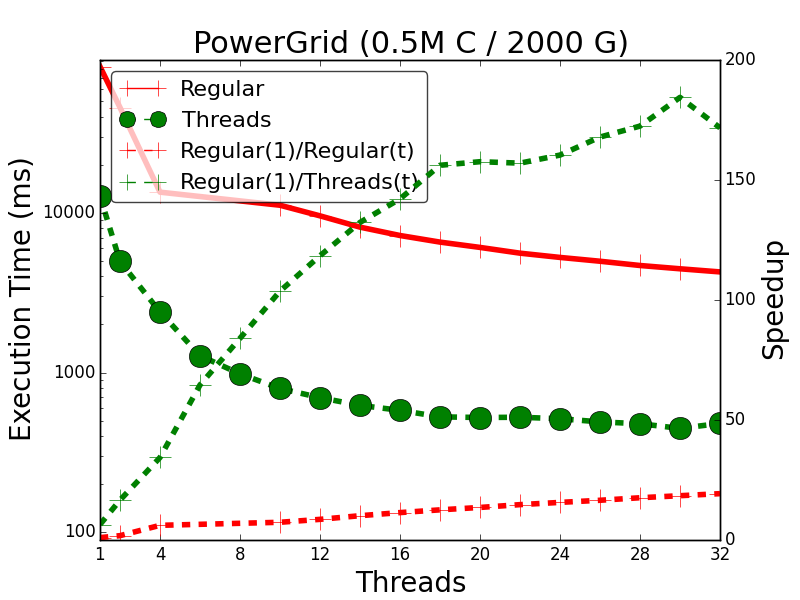
\includegraphics[width=\textwidth]{experiments/threads/cmp-powergrid-500000C2000G.png}
           \caption{}
           \label{fig:threads:powergrid1}
        \end{subfigure}
        ~
        \begin{subfigure}[b]{\plotsize\textwidth}
           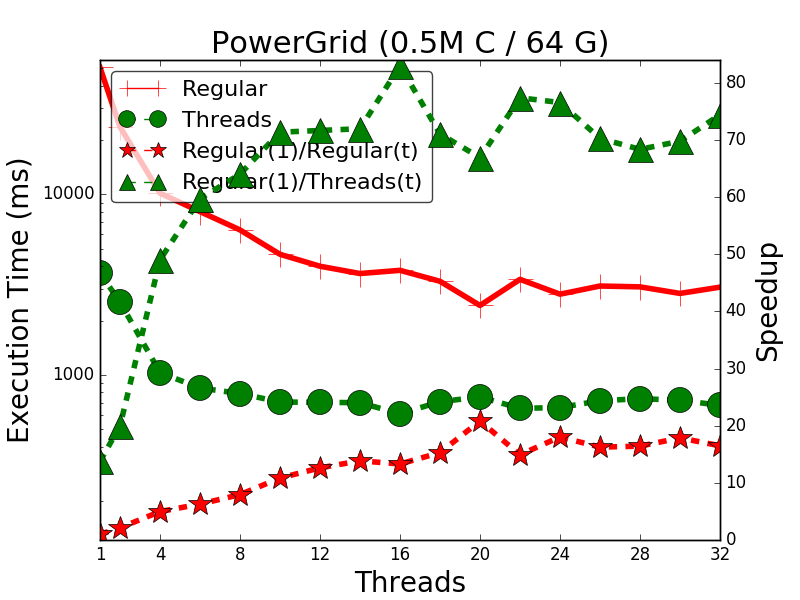
\includegraphics[width=\textwidth]{experiments/threads/cmp-powergrid-500000C64G.png}
           \caption{}
           \label{fig:threads:powergrid2}
        \end{subfigure} \\
        \begin{subfigure}[b]{\plotsize\textwidth}
           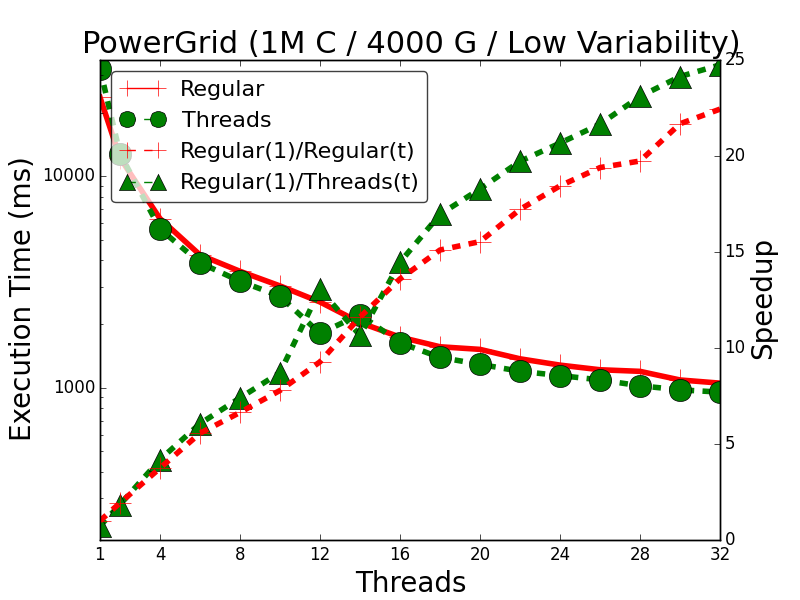
\includegraphics[width=\textwidth]{experiments/threads/cmp-powergrid-1M4000C-low.png}
           \caption{}
           \label{fig:threads:powergrid3}
        \end{subfigure} ~
        \begin{subfigure}[b]{\plotsize\textwidth}
           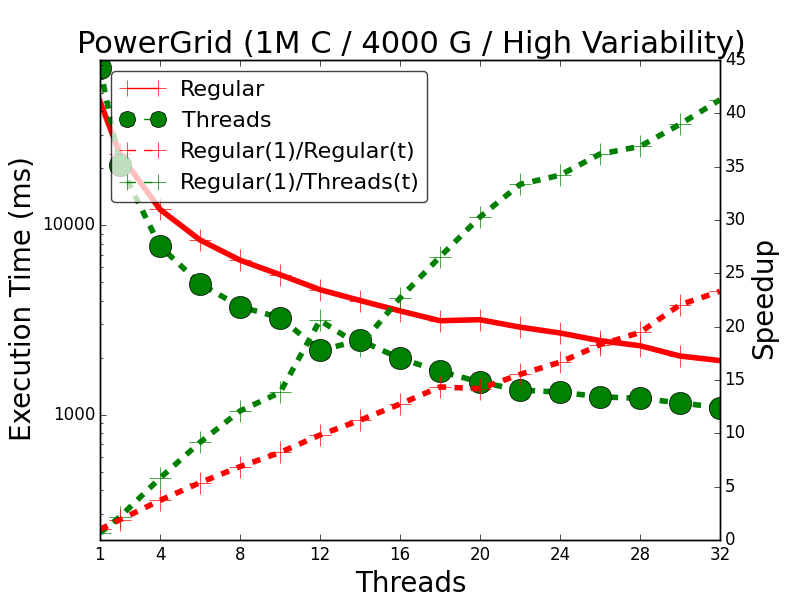
\includegraphics[width=\textwidth]{experiments/threads/cmp-powergrid-1M4000C-high.png}
           \caption{}
           \label{fig:threads:powergrid4}
        \end{subfigure} \\
        \caption{Measuring the performance of the PowerGrid program
        when using thread facts.}
        \label{fig:threads:results_powergrid}
\end{figure}

The second important observation relates to the last two datasets where we
experimented with a variable capacity for the generators. For the Low
Variability dataset, the consumers have very identical capacities, while in the
High Variability dataset, generators have a more variable capacity, which should
make it harder for the algorithm to find a valid generator/consumer assignment.
Our results show exactly that: the Low Variability shows a very small difference
between the \textbf{Regular} and \textbf{Threads} version, while in the High
Variability dataset, the \textbf{Threads} version is much faster than the
\textbf{Regular} version. However, for the High Variability dataset, we were
expecting a speedup that was closer to the 0.5 M C / 2000 G dataset, since the
number of generators is much higher. Furthermore, if we compare the run times of
the \textbf{Regular} and \textbf{Threads} version when using 1 thread, we notice
that the \textbf{Threads} version is actually slower. As noted before, this may
be due to the fact that the LM rule for assigning generators to consumers needs
to perform a linear scan on the available generators to find a suitable
generator which then negatively impacts performance. This is a clear drawback of
the logic programming model that could potentially be solved by maintaining a
sorted list of \texttt{thread-capacity} facts.

In Table~\ref{table:threads:powergrid_stats}, we present several fact statistics
that compare the \textbf{Regular} version with the \textbf{Threads} version when
executing with multiple threads. The \textbf{\# Derived} column indicates the
number of derived facts, \textbf{\# Deleted} indicates the number of retracted
facts, while \textbf{\# Final} is the number of facts in the database after the
program terminates. The table results clearly show that using thread-based facts
results in a decrease in the number of generated facts, which is more
significant in the 0.5M C / 2000 G dataset (10-fold reduction). The table also
explains why this dataset performs much better than the 1M C / 4000 G High
Variability dataset, which only sees a 2-fold reduction in derived facts.

When comparing the number of facts derived when using a different number of
threads, the overall trend indicates that having more threads slightly increases
the number of derived facts. This is especially true for the 0.5 M C / 64 G
datasets, where twice as many facts are generated when using 32 threads when
compared to 1 thread.

\begin{table}[ht]
   \begin{center}
      \begin{tabular}{c | c || c c | c c | c c} \hline
	 \multirow{2}{*}{\textbf{Dataset}} & \multirow{2}{*}{\textbf{Threads}} & \multicolumn{2}{c|}{\textbf{\# Derived}} & \multicolumn{2}{c|}{\textbf{\# Deleted}} & \multicolumn{2}{c}{\textbf{\# Final}}\\
	 & & Regular & Threads & Regular & Threads & Regular & Threads\\ \hline \hline
\multirow{7}{*}{0.5M C / 2000 G}  & 1 &  49.7M & 4.2M &  48.2M & 2.5M &  2.5M & 2.5M \\
 & 2 &  48.5M & 4.4M &  47.7M & 2.5M &  2.5M & 2.5M \\
 & 4 &  49.4M & 4.1M &  47.9M & 2.6M &  2.5M & 2.5M \\
 & 8 &  49.4M & 4.10M &  47.9M & 2.5M &  2.5M & 2.5M \\
 & 16 &  50.8M & 4.1M &  49.3M & 2.6M &  2.5M & 2.5M \\
 & 24 &  49.8M & 4.2M &  48.3M & 2.7M &  2.5M & 2.5M \\
 & 32 &  49.3M & 4.6M &  47.8M & 3.1M &  2.5M & 2.5M \\
	\hline
\multirow{7}{*}{0.5M C / 64 G}  & 1 &  20.2M & 4.3M &  18.5M & 2.5M &  2.5M & 2.5M \\
 & 2 &  19.9M & 4.2M &  18.4M & 2.7M &  2.5M & 2.5M \\
 & 4 &  20.7M & 4.4M &  18.5M & 2.9M &  2.5M & 2.5M \\
 & 8 &  19.9M & 5.6M &  18.4M & 4.10M &  2.5M & 2.5M \\
 & 16 &  19.8M & 6.8M &  18.3M & 5.3M &  2.5M & 2.5M \\
 & 24 &  19.7M & 8.4M &  18.2M & 6.9M &  2.5M & 2.5M \\
 & 32 &  19.9M & 9.3M &  18.4M & 7.5M &  2.5M & 2.5M \\
	\hline
\multirow{7}{*}{\makecell{1M C / 4000 G \\Low Variability}}  & 1 &  9.4M & 7.5M &  6.4M & 4.5M &  5.1M & 5.1M \\
 & 2 &  9.4M & 7.5M &  6.4M & 4.5M &  5.1M & 5.1M \\
 & 4 &  9.4M & 7.5M &  6.4M & 4.5M &  5.1M & 5.1M \\
 & 8 &  9.4M & 7.6M &  6.4M & 4.6M &  5.1M & 5.1M \\
 & 16 &  9.4M & 7.5M &  6.4M & 4.5M &  5.1M & 5.1M \\
 & 24 &  9.4M & 7.6M &  6.3M & 4.6M &  5.1M & 5.1M \\
 & 32 &  9.3M & 7.5M &  6.3M & 4.5M &  5.1M & 5.1M \\
	\hline
\multirow{7}{*}{\makecell{1M C / 4000 G \\High Variability}}  & 1 &  16.4M & 8.8M &  13.4M & 5.8M &  5.1M & 5.1M \\
 & 2 &  16.5M & 8.8M &  13.5M & 5.8M &  5.1M & 5.1M \\
 & 4 &  16.5M & 8.8M &  13.4M & 5.8M &  5.1M & 5.1M \\
 & 8 &  16.5M & 8.9M &  13.5M & 5.9M &  5.1M & 5.1M \\
 & 16 &  16.5M & 8.8M &  13.5M & 5.8M &  5.1M & 5.1M \\
 & 24 &  16.5M & 9.3M &  13.5M & 6.2M &  5.1M & 5.1M \\
 & 32 &  16.5M & 9.6M &  13.5M & 6.5M &  5.1M & 5.1M \\
	\hline
\end{tabular}

   \end{center}

   \caption{Measuring the reduction in derived facts when using thread-based
   facts.}
   \label{table:threads:powergrid_stats}
\end{table}

%\clearpage
